\subsection{Image filtering}
Our last experiment consists in applying some filters to a selection of 18 ImageNet images to evaluate possible changes in the image colorization output. We considered a blurring filter with kernel sizes of 3, 7 or 11, a cartoonizing filter from \cite{cartoonize} and the increasing or decreasing of contrast and luminance.

In general, a blurred image is harder to colorize, and the more blurred the image is, the worse
the final colorization we get. Indeed, in the example reported Figure \ref{fig:filter} the dogs have some weird pink/orange
spots on their fur.
On the contrary, images with a higher contrast and luminance get a better colorization
by all the models, with just a few exceptions depending on the specific image.

Clearly, with cartoonization we reach very unrealistic colors. In the example, it looks like the model
didn't recognize the grass and probably mistook it for water. Probably, this is not due to the fact that cartoonization discards some details from the original images, because blurring does the same. This could be rather due to the fact that the models are not trained on cartoonized images and expect a completely different "image stile" in input. 

In conclusion, Figure \ref{fig:filter} is a good example of how the colorization is an ambiguous task: the model colors the grass with a plausible green tone, which actually could result more realistic than the original brown tone.

\begin{figure*}[ht]
	\centering
	\captionsetup[subfigure]{labelformat=empty}
		\begin{subfigure}[b]{0.1\textwidth}
		\centering
		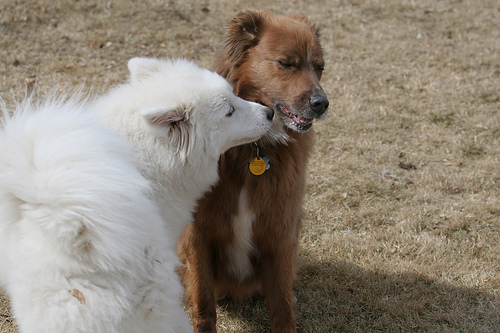
\includegraphics[width=2.4cm]{orig - filter.jpeg}
		\caption{Original}
		\end{subfigure}
		\hfill
		\begin{subfigure}[b]{0.1\textwidth}
			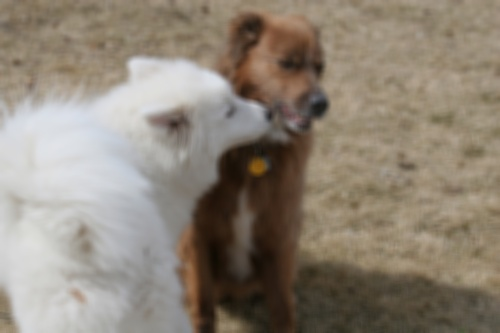
\includegraphics[width=2.4cm]{orig - filter - blur.jpeg}
			\caption{Blurred}
		\end{subfigure}
		\hfill
		\begin{subfigure}[b]{0.1\textwidth}
			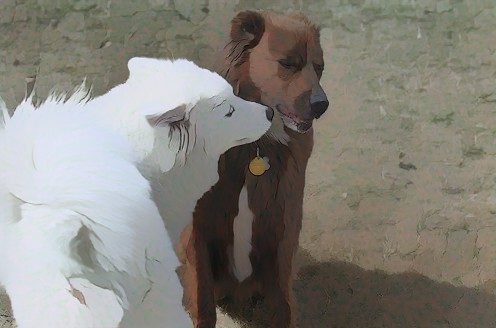
\includegraphics[width=2.4cm]{orig - filter - cartoon.jpeg}
			\caption{Cartoon}
		\end{subfigure}
		\hfill
		\begin{subfigure}[b]{0.1\textwidth}
			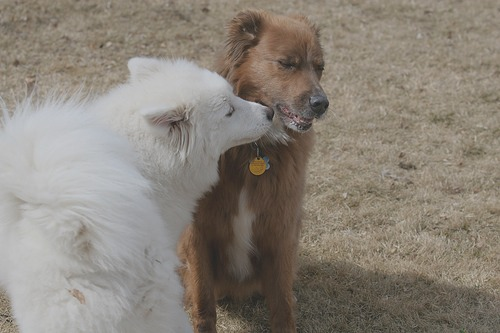
\includegraphics[width=2.4cm]{orig - filter - man contr (2).jpg}
			\caption{Low contrast}
		\end{subfigure}
		\hfill
		\begin{subfigure}[b]{0.1\textwidth}
			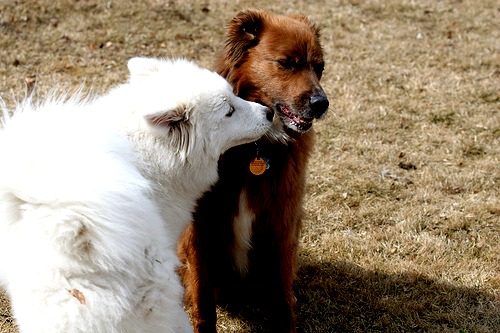
\includegraphics[width=2.4cm]{orig - filter - man contr (1).jpg}
			\caption{High contrast}
		\end{subfigure}
		\hfill
		\begin{subfigure}[b]{0.1\textwidth}
			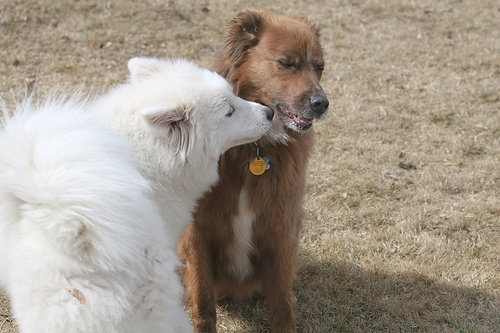
\includegraphics[width=2.4cm]{orig - filter - lumin (1).jpeg}
			\caption{Brighter}
		\end{subfigure}
		\hfill
		\begin{subfigure}[b]{0.1\textwidth}
			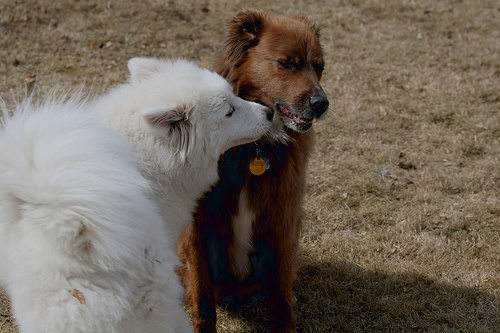
\includegraphics[width=2.4cm]{orig - filter - lumin (2).jpeg}
			\caption{Darker}
		\end{subfigure}
	
				\begin{subfigure}[b]{0.1\textwidth}
			\centering
			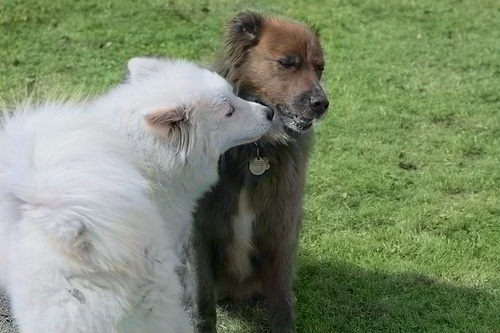
\includegraphics[width=2.4cm]{c - filter.jpeg}

		\end{subfigure}
		\hfill
		\begin{subfigure}[b]{0.1\textwidth}
			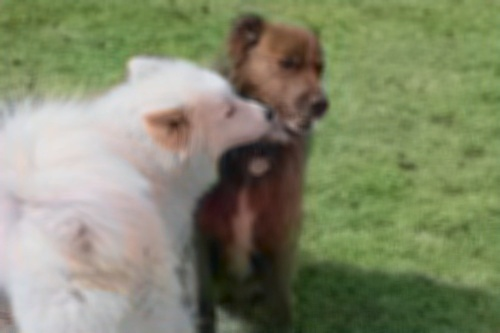
\includegraphics[width=2.4cm]{c - filter - blurr.jpeg}
		\end{subfigure}
		\hfill
		\begin{subfigure}[b]{0.1\textwidth}
			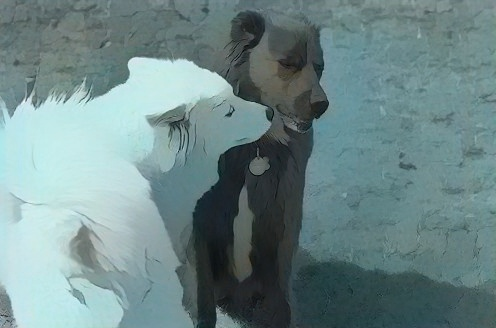
\includegraphics[width=2.4cm]{c - filter - cartoon.jpeg}
		
		\end{subfigure}
		\hfill
		\begin{subfigure}[b]{0.1\textwidth}
			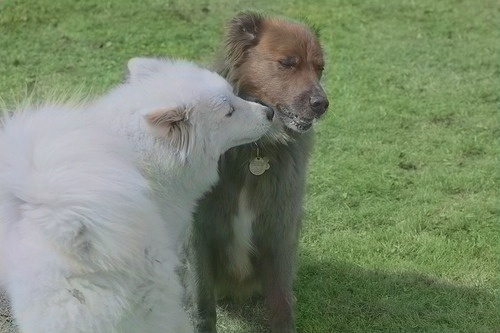
\includegraphics[width=2.4cm]{c - filter - man contr (1).jpg}
	
		\end{subfigure}
		\hfill
		\begin{subfigure}[b]{0.1\textwidth}
			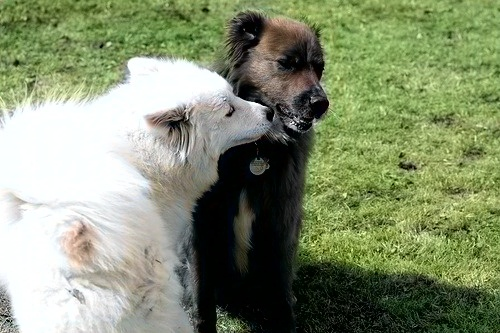
\includegraphics[width=2.4cm]{c - filter - man contr (2).jpg}
	
		\end{subfigure}
		\hfill
		\begin{subfigure}[b]{0.1\textwidth}
			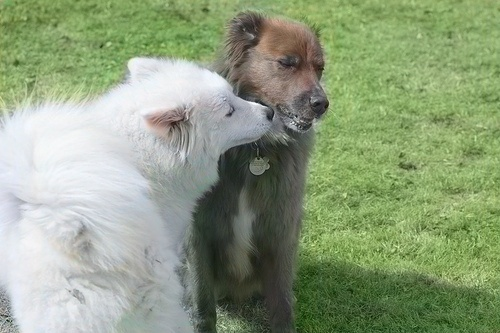
\includegraphics[width=2.4cm]{c - filter - lumin (1).jpeg}
	
		\end{subfigure}
		\hfill
		\begin{subfigure}[b]{0.1\textwidth}
			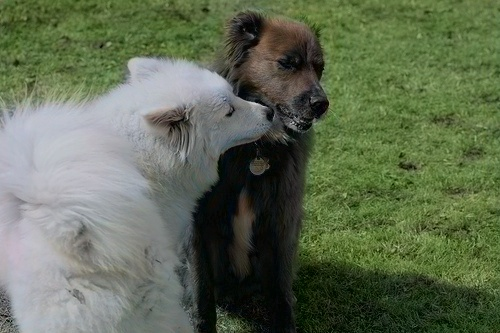
\includegraphics[width=2.4cm]{c - filter - lumin (2).jpeg}
	
		\end{subfigure}
	\caption{{\small ChromaGAN colorization (second row) on some filtered images (first row).}}
	\label{fig:filter}
\end{figure*}